\documentclass{exam}
\printanswers
\usepackage{times}
\usepackage[T1]{fontenc}
\usepackage[portuges]{babel}


% Comentar para not MAC Users
\usepackage[utf8]{inputenc}

\usepackage{a4}
%\usepackage[margin=3cm,nohead]{geometry}
\usepackage{epstopdf}
\usepackage{graphicx}
\usepackage{fancyvrb}
\usepackage{amsmath}
\usepackage{float}
%\renewcommand{\baselinestretch}{1.5}



\begin{document}
\title{Redes Sem Fios (802.11)}

\author{Etienne Costa(A76089) \and Joana Cruz(A76270) \and Rafael Alves(A72629)}

\date{}
\maketitle

\begin{abstract}
Este Trabalho tem como objectivo explorar vários aspectos do protocolo IEEE 802.11, tais comom o formato das tramas, o edenreçamentos dos componentes envolvidos na comunicação sem fios, os tipos de tramas mais comuns, bem como a operação do protocolo.
\end{abstract}
\section{Acesso Rádio}

\begin{questions}
\question Identifique em que frequência do espectro está a operar a rede sem fios, e o canal que corresponde essa frequência.
\begin{solution}
A rede sem fios está a operar a uma frequência de \underline{2467 MHz}, sendo que essa frequência corresponde ao canal \underline{12}.
\end{solution}

\question Identifique a versão da norma IEEE 802.11 que está a ser usada.
\begin{solution}
A versão da norma IEEE 802.11 que está a ser utilizada é a \underline{802.11g}. 
\end{solution}

% Perguntar se querem o débito máximo desta versão em particular? Pois se for o valor é 54 Mbs
\question Qual o débito a que foi enviada a trama escolhida? Será que esse débito corresponde ao débito máximo a que a interface Wifi pode operar? Justifique.
\begin{solution}
A trama escolhida foi enviada com um débito de \underline{1,0 Mb/s}. Não, visto que o débito máximo que a interface Wifi pode operar são \underline{54 Mbp/s}.
\end{solution}

\begin{figure}[H]
\centering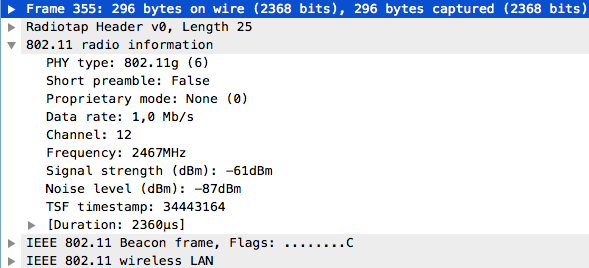
\includegraphics[scale=0.50]{Trama355} 
\caption{\label{fig:controller}Trama 355}
\end{figure}

\end{questions}

\section{Scanning Passivo e Scanning Ativo}

\begin{questions}
\question Selecione uma trama beacon(e.g., a trama 3xx) Esta trama pertence a que tipo de tramas 802.11? Indique o valor dos seus identificadores de tipo e subtipo.
Em que parte concreta do cabeçalho da trama estão especificados (ver anexo)?
\begin{solution}
A figura 2 corresponde a trama selecionada, como podemos constatar na imagem podemos afirmar que é uma management frames ou seja tramas de gestão.
Os valores dos seus identificadores de tipo e subtipo são os seguinte:
\begin{equation}
\textbf{Type}:0
\end{equation} 
\begin{equation}
\textbf{Subtype}:8
\end{equation} 
Estes valores podem ser encontrados no cabeçalho Frame Control Field.
\end{solution}

\question Liste todos os SSIDs dos APs (Access Points) que estão a operar na vizinhança da STA de captura? Explicite o modo como obteve essa informação.Como sugestão pode construir um filtro de visualização apropriado (tomando como base a resposta da alínea anterior) que lhe permita obter a listagem pretendida.
\begin{solution}
Sendo que os SSIds estão contidos nas tramas de gestão cujo  valor do seu identificador de tipo é igual a 0 utilizamos o seguinte comando para filtrar
as respectivas tramas de gestão.
\begin{equation}
wlan.fc.type==0
\end{equation}
De modo a filtrar os SSIDs dos APs que estão a operar na vizinhança da STA de captura necessitamos de filtrar as tramas de gestão cujo valor do identificador de subtipo é igual a 1 que por sua vez corresponde as tramas de anúncio (Beacon) utilizamos o seguinte comando para filtrar.
\begin{equation}
wlan.fc.subtype==8
\end{equation}
Fundindo os dois comando conseguimos listar os seguintes SSIDs:
\begin{description}
	\item[•] \verb|FlyingNet|. 
	\item[•] \verb|NOS_WIFI_Fon|.
\end{description}
\end{solution}
\begin{figure}[H]
\flushleft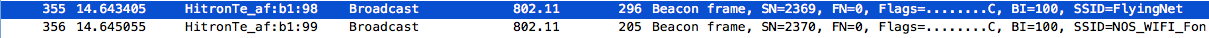
\includegraphics[scale=0.35]{SSIDs} 
\caption{\label{fig:controller}SSIDs Listados.}
\end{figure}



\question Verifique se está a ser usado o método de detecção de erros (CRC), e se todas as tramas Beacon recebidas corretamente. Justifique o porquê de usar detecção de erros neste tipo de redes locais.
\begin{solution}
Podemos afirmar que está a ser usado o método de detecção de erros e que as tramas Beacon estão a ser recebidas corretamente visto que 
o status da frame check sequence é GOOD. A detecção de erros é usada neste tipo de redes locais pois a probabilidade de ocorrência de colisões é muito elevada levando assim a uma grande ocorrência de erros.
\end{solution}


\question Para dois dos APs identificados, indique qual é o intervalo de tempo previsto entre tramas beacon consecutivas? (Nota: este valor é anunciado na própria trama beacon). Na prática, a periodicidade de tramas beacon é verificada? Tente explicar porquê.
\begin{solution}
O intervalo de tempo previsto entre tramas beacon consecutivas é 0.1024 segundos.
Na prática a periodicidade de tramas beacon não é verificada devido as colisões que ocorrem , algumas tramas são adiadas.

\begin{figure}[H]
\centering
\includegraphics[scale=0.45]{BeaconInterval} 
\caption{\label{fig:controller}Beacon Interval}
\end{figure}
\end{solution}

\question Identifique e registe todos os endereços MAC usados nas tramas beacon enviadas pelos APs. Recorde que o endereçamento está definido no cabeçalho das tramas 802.11, podendo ser utilizados até quatro endereços com diferente semântica. Para uma descrição detalhada da estrutura da trama 802.11, consulte o anexo ao enunciado.
\begin{solution}
O endereço MAC cujo SSID do AP é \verb|Flyingnet| é o:\textbf{bc:14:01:af:b1:98}
\begin{figure}[H]
\centering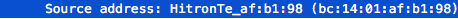
\includegraphics[scale=0.45]{MAC1} 
\caption{\label{fig:controller}SSID:FlyingNet}
\end{figure}
O endereço MAC cujo SSID do AP é \verb|NOS_WIFI_Fon| é o :\textbf{bc:14:01:af:b1:99}
\begin{figure}[H]
\centering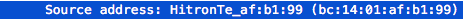
\includegraphics[scale=0.45]{MAC2} 
\caption{\label{fig:controller}SSID:NOS WIFI Fon}
\end{figure}

\end{solution}

\question As tramas beacon anunciam que o AP pode suportar vários débitos de base assim como vários "extended supported rates". Indique quais são esses débitos?
\begin{solution}
Os vários débitos de base que o AP pode suportar são:
\begin{figure}[H]
\centering
\includegraphics[scale=0.45]{SupportedRates} 
\caption{\label{fig:controller}Supported Rates}
\end{figure}

Os vários extended supported rates são:
\begin{figure}[H]
\centering
\includegraphics[scale=0.45]{ExtendSuportedRates} 
\caption{\label{fig:controller}Supported Rates}
\end{figure}

\end{solution}

\question Estabeleça um filtro Wireshark apropriado que lhe permita visualizar todas as tramas probing request ou probing response,simultaneamente.
\begin{solution}
Visto que os valores dos identificadores de subtipos de tramas probing  request e reply são 4 e 5 temos o seguinte filtro:
\begin{equation}
wlan.fc.type==0 \&\& ( wlan.fc.subtype==4 || wlan.fc.subtype==5)
\end{equation}
\end{solution}


\begin{figure}[H]
\centering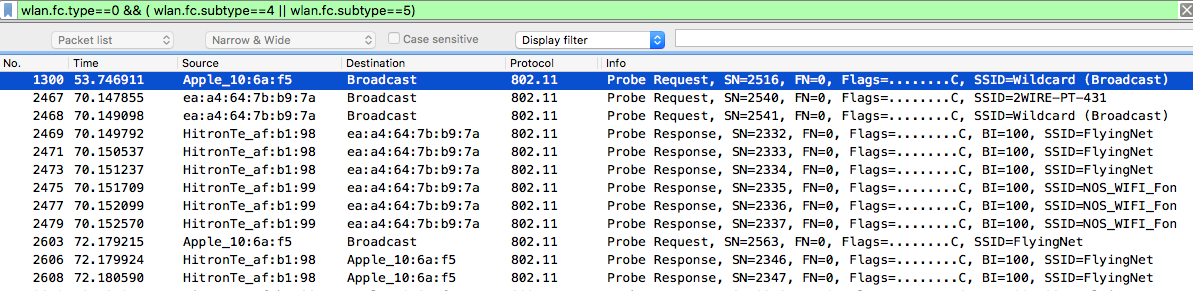
\includegraphics[scale=0.40]{ProbeRequestResponse} 
\caption{\label{fig:controller}Probe Request e Probe Response}
\end{figure}



\question Identifique um probing request para o qual tenha havido um probing response.Face ao endereçamento usado, indique a que sistemas são endereçadas estas tramas e explique qual o propósito das mesmas?
\begin{solution}
Quando uma STA está a procura de uma rede, ela envia uma trama chamada probe request, contendo o SSID da rede que ela procura. O AP que tiver o
SSID em questão, envia o probe response. Com base nisso  Temos a STA (Apple\_10:6a:f5) que envia uma trama probe request com o SSID igual a FlyingNet em broadcast ou seja para todos os APs. Uma vez que o AP(HitronTe\_af:b1:98) com o SSID específico foi encontrado, a estação inicia os passos de autenticação e associação
para entrar na rede através deste AP.
\end{solution}

\begin{figure}[H]
\centering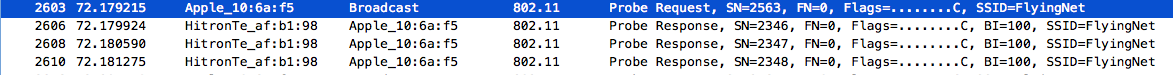
\includegraphics[scale=0.40]{ProbingRequestHaveResponse} 
\caption{\label{fig:controller}Probe Request com Probe Response}
\end{figure}



\begin{figure}[H]
\centering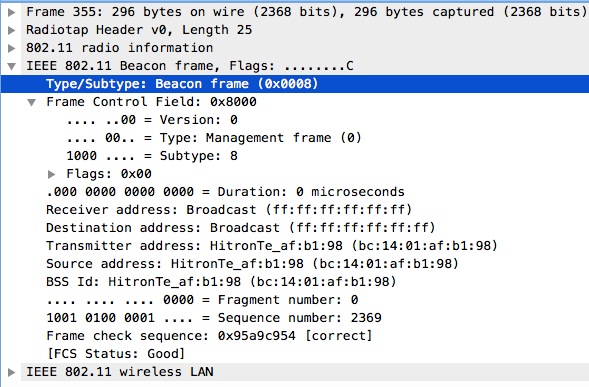
\includegraphics[scale=0.50]{TramaBeacon355} 
\caption{\label{fig:controller}Trama Beacon 355}
\end{figure}

\end{questions}


\section{Processo de Associação}
\begin{questions}
\question Identifique uma sequência de tramas que corresponda a um processo de associação completo entre a STA e o AP, incluindo a fase de autenticação.
\begin{figure}[H]
\centering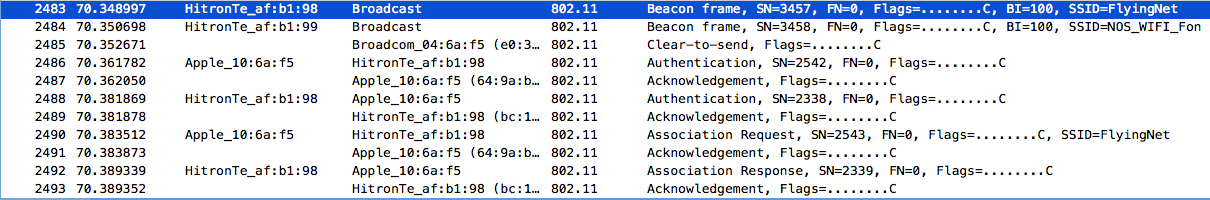
\includegraphics[scale=0.40]{Authentication} 
\caption{\label{fig:controller}Processo de associação completo.}
\end{figure}


\question Efetue um diagrama que ilustre a sequência de todas as tramas trocadas no processo.
\begin{figure}[H]
\centering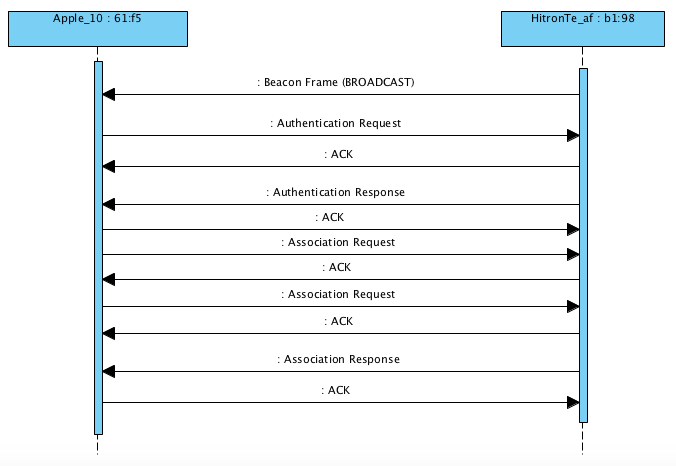
\includegraphics[scale=0.45]{TramasTrocadas} 
\caption{\label{fig:controller}Sequência de tramas trocadas.}
\end{figure}
\end{questions}

\section{Transferência de Dados}

\begin{questions}

\question Considere a trama de dados nº455.Sabendo que o campo Frame Control contido no cabeçalho das tramas 802.11 permite especificar a direccionalidade das tramas,o que pode concluir face à direccionalidade dessa trama, será local à WLAN?
\begin{solution}
Nesta trama a direccionalidade é :
Frame from DS to a STA via AP (To Ds: 0 From Ds: 1).
\end{solution}

\question Para a trama de dados nº455, transcreva os endereços MAC em uso identificando qual o endereço MAC correspondente ao host sem fios (STA), ao AP e ao router de acesso ao sistema de distribuição?
\begin{solution}

MAC STA (Receiver Adress)  : d8:a2:5e:71:41:a1.

MAC AP (Transmitter Adress): bc:14:01:af:b1:98.

MAC Router (Source Adress) : bc:14:01:af:b1:98.

\end{solution}
\begin{figure}[H]
\centering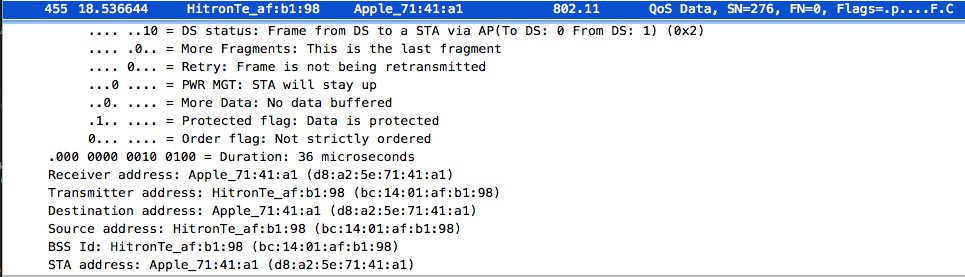
\includegraphics[scale=0.45]{direcionalidade455} 
\caption{\label{fig:controller}Frame 455 Adressing}
\end{figure}


\question Como interpreta a trama nº457 face à sua direccionalidade e endereçamento MAC?
\begin{solution}
Nesta trama a direccionalidade é :
Frame from DS to a STA via AP (To Ds: 1 From Ds: 0).


MAC Router (Destination Adress)  : bc:14:01:af:b1:98.

MAC STA (Source Adress): d8:a2:5e:71:41:a1.

MAC AP (Receiver Adress) : bc:14:01:af:b1:98.
\end{solution}

\begin{figure}[H]
\centering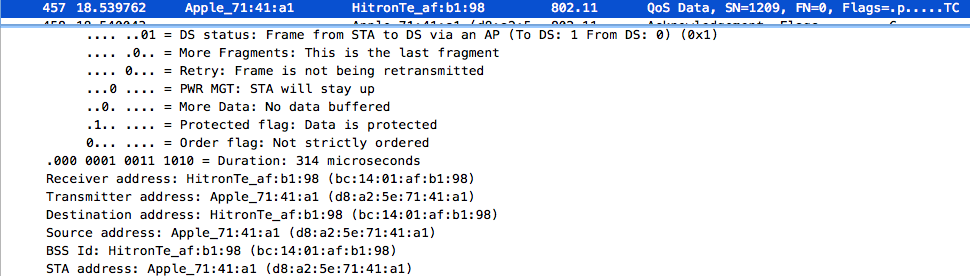
\includegraphics[scale=0.45]{direcionalidade457} 
\caption{\label{fig:controller}Frame 457 Adressing}
\end{figure}


\question Que subtipo de tramas de controlo são transmitidas ao longo da transferência de dados acima mencionada? Tente explicar porque razão têm de existir (contrariamente ao que acontece numa rede Ethernet.)
\begin{solution}
O subtipo de tramas de controlo transmitidas ao longo da transferência de dados acima menciona é a Acknowlegment ou seja trama de confirmação da recepção.
Elas têm que existir de modo a ser possível fazer a deteção de erros, sendo que quando não são encontrados erros é enviada uma Trama ACK para a STA emissora.
\end{solution}

\question O uso de trama Request To Send e Clear To Send, apesar de opcional, é comum para efetuar "pré-reserva" do acesso ao meio quando se pretende enviar tramas de dados, com o intuito de reduzir o número de colisões resultante maioritariamente de STAs escondidas. Para o exemplo acima,verifique se está a ser usada a opção RTS/CTS na troca de dados entre a STA e o AP/Router da WLAN, identificando a direccionalidade das tramas e os sistemas envolvidos.
\begin{solution}
Relativamente a direcionalidade visto que estamos perante a tramas de dados os valores da direcionalidade serão sempre 
(To DS:0 From DS:0).
\begin{description}
	\item[•] \verb|STA:Apple_10:6a:f5|. 
	\item[•] \verb|AP:HitronTe_af:b1:98|.
\end{description}

\end{solution}
\begin{figure}[H]
\centering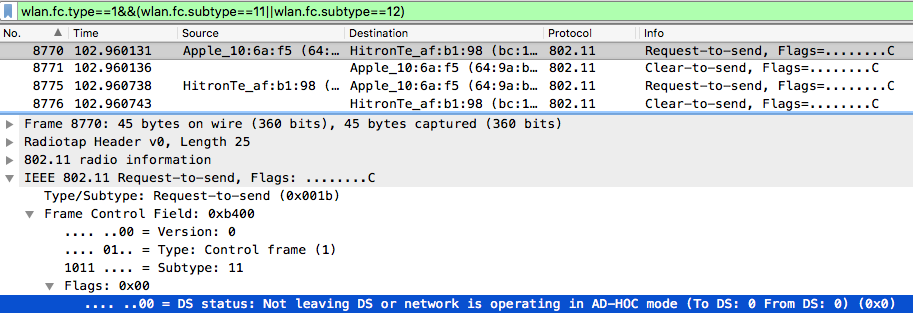
\includegraphics[scale=0.45]{18} 
\caption{\label{fig:controller}Tramas Request To Sent e Clear To Send}
\end{figure}
\end{questions}

\section{Conclusão}
O protocolo de comunicação sem fios 802.11, dado as caraterísticas do meio, exige uma implementação mais complexa do que o protocolo Ethernet anteriormente estudado. Este facto leva a existência de tramas com cabeçalhos mais complexos e de tamanho superior, que desempenham funções de controlo de erros e garantem a estabilidade das conexões. Uma das formas de garantir esta propriedade  é através das tramas Beacon enviadas pelos APs que permitem que as stations optem pelo AP mais favorável. O processo de estabelecimento de uma conexão sem fios  é conhecido por Associação, sendo precedido de uma fase de autenticação da station por parte do AP que rejeita ou aceita a identidade do primeiro. A transmissão de dados em redes sem fios  é auxiliada pela troca de tramas de Acknowlegment(ACK) que confirmam a receção (correta) de uma determinada trama, sendo por vezes precedidas de tramas RTS e CTS que têm o intuito de prevenir a ocorrência de colisões durante a transmissão.

\end{document}